\chapter{Optique}

\section{Explications sur le télescope de Dobson}

Le télescope est un instrument permettant d'observer le ciel en amplifiant la lumière captée des astres et en agrandissant l'image vue. Il réalise cela par un jeu de miroirs, à la différence de la lunette astronomique qui utilise un jeu de lentilles.

Il existe plusieurs types de télescope, celui de Newton est composé d'un miroir parabolique "primaire" concentrant la lumière vers un miroir plan "secondaire" la déviant vers l'oculaire, où l'utilisateur place son œil.

\begin{figure}[H]
    \centering
    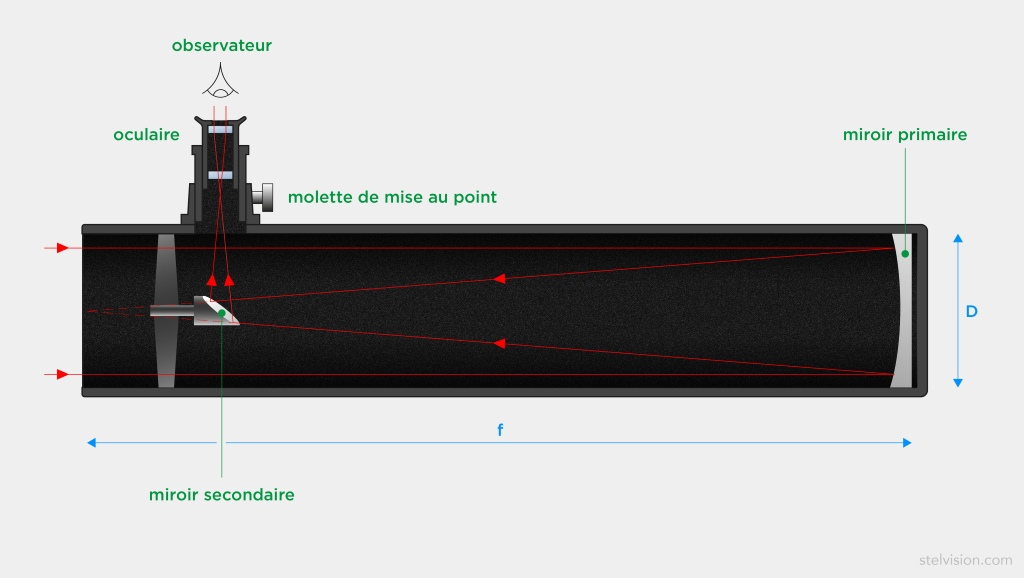
\includegraphics[width=0.9\linewidth]{\figures/sch_newton.jpg}
    \decoRule
    \caption[
    Schéma du télescope de Newton\\(Schéma \textcopyright Stelvision)]{
    Schéma du télescope de Newton\\(Schéma \textcopyright Stelvision)}
    \label{fig:Schéma du télescope de Newton (Schéma copyright Stelvision)}
    \end{figure}

\vspace{1cm}

L'amplification lumineuse dépend du diamètre $D$ du miroir parabolique. Le grossissement dépend de la distance focale de la parabole $f$. Le diamètre détermine la luminosité et la finesse de l'image. La distance focale détermine le grossissement. Trop agrandir l'image par augmentation de la distance focale assombrit et dégrade sa qualité.

\vspace{1cm}

Le télescope de Dobson est un télescope de Newton doté d'une monture azimutale simplifiée. Il a été inventé par un astronome amateur et a les avantages d'être simple de fabrication et relativement peu onéreux pour un télescope.

\begin{figure}[H]
    \centering
    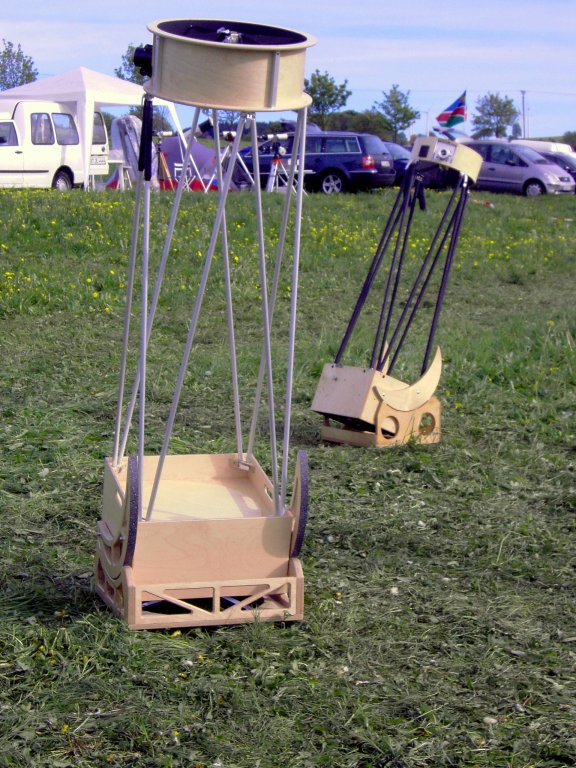
\includegraphics[width=0.45\linewidth]{\figures/photo_dobson_1.jpg}
    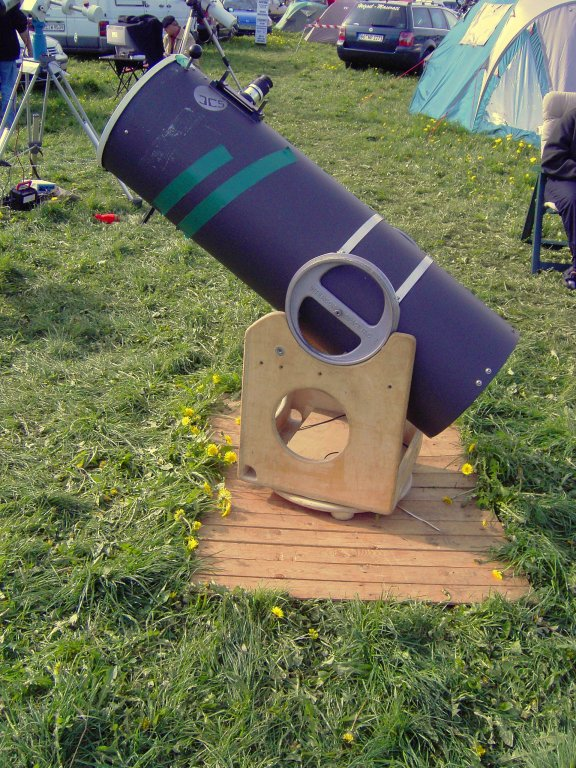
\includegraphics[width=0.45\linewidth]{\figures/photo_dobson_2.jpg}
    \decoRule
    \caption[
    Télescopes de Dobson]{
    Télescopes de Dobson}
    \label{fig:Télescopes de Dobson}
    \end{figure}

\section{Choix de l'oculaire}

L'oculaire d'un télescope est un jeu de lentilles placé au plan focal de l'image produite par celui-ci. Il sert avant tout à faire de cette image présente au plan focal une image "à l'infini", c'est-à-dire nette sans accommodation de l'œil. Il permet également, par sa propre distance focale, d'ajuster le grossissement du télescope.

\begin{align*}
G&=\frac{f_{miroir primaire}}{f_{oculaire}}
\end{align*}

\vspace{1cm}

Un zoom est un objectif à lentilles mobiles et à distance focale variable. Il permet donc d'ajuster l'angle d'ouverture de l'appareil et de modifier son grossissement. Il existe des oculaires zoom pour télescope.

\vspace{1cm}

Le site internet Stelvision met à disposition un simulateur d'oculaires. Il permet, pour un télescope de caractéristiques $f$ et $D$ données, de visualiser l'image produite avec des oculaires de distances focales différentes. Quelques astres sont observables.

\url{https://www.stelvision.com/simulateur-telescope/simulateur-telescope.php}

\vspace{1cm}

Les caractéristiques de l'Autoscope sont les suivantes~:

\begin{align*}
D&=254mm&f&=1,27m
\end{align*}

\begin{figure}[H]
    \centering
    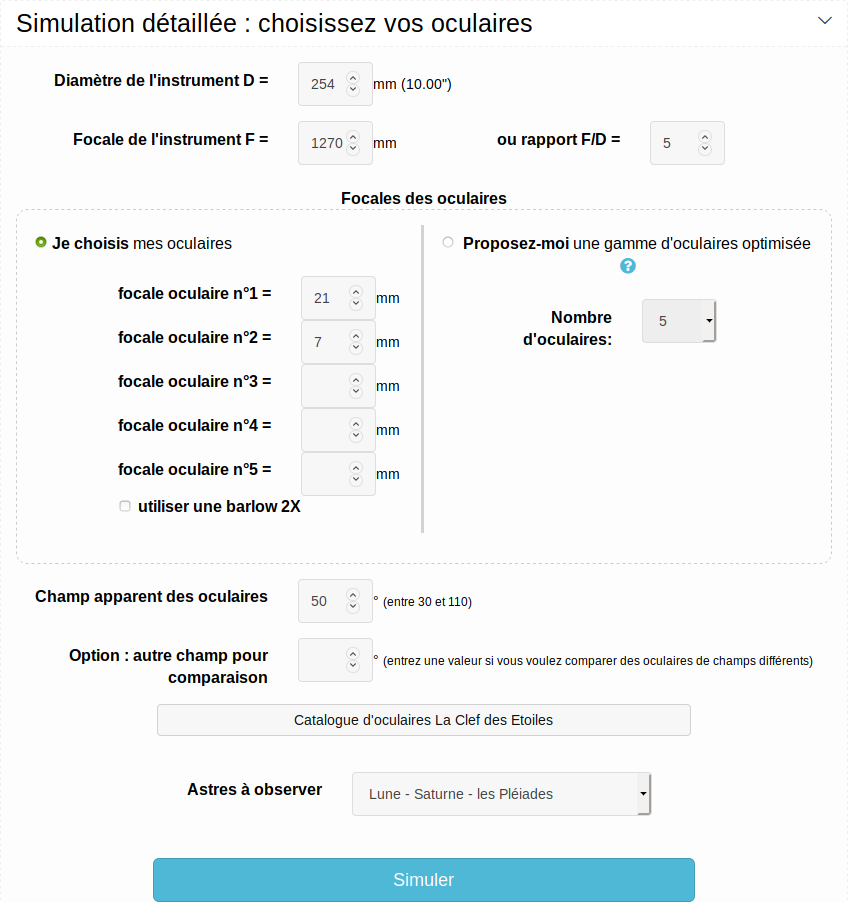
\includegraphics[width=0.9\linewidth]{\figures/photo_stelvision1.png}
    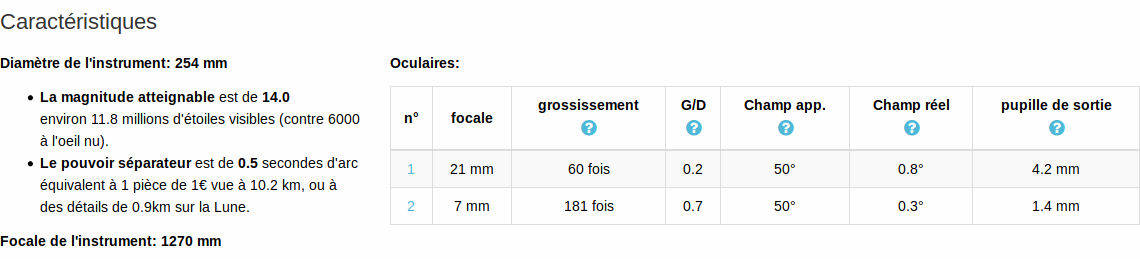
\includegraphics[width=1\linewidth]{\figures/photo_stelvision2.png}
    \decoRule
    \caption[
	Simulateur de télescope Stelvision.com]{
    Simulateur de télescope Stelvision.com}
    \label{fig:Simulateur de télescope Stelvision.com}
    \end{figure}

\begin{figure}[H]
    \centering
    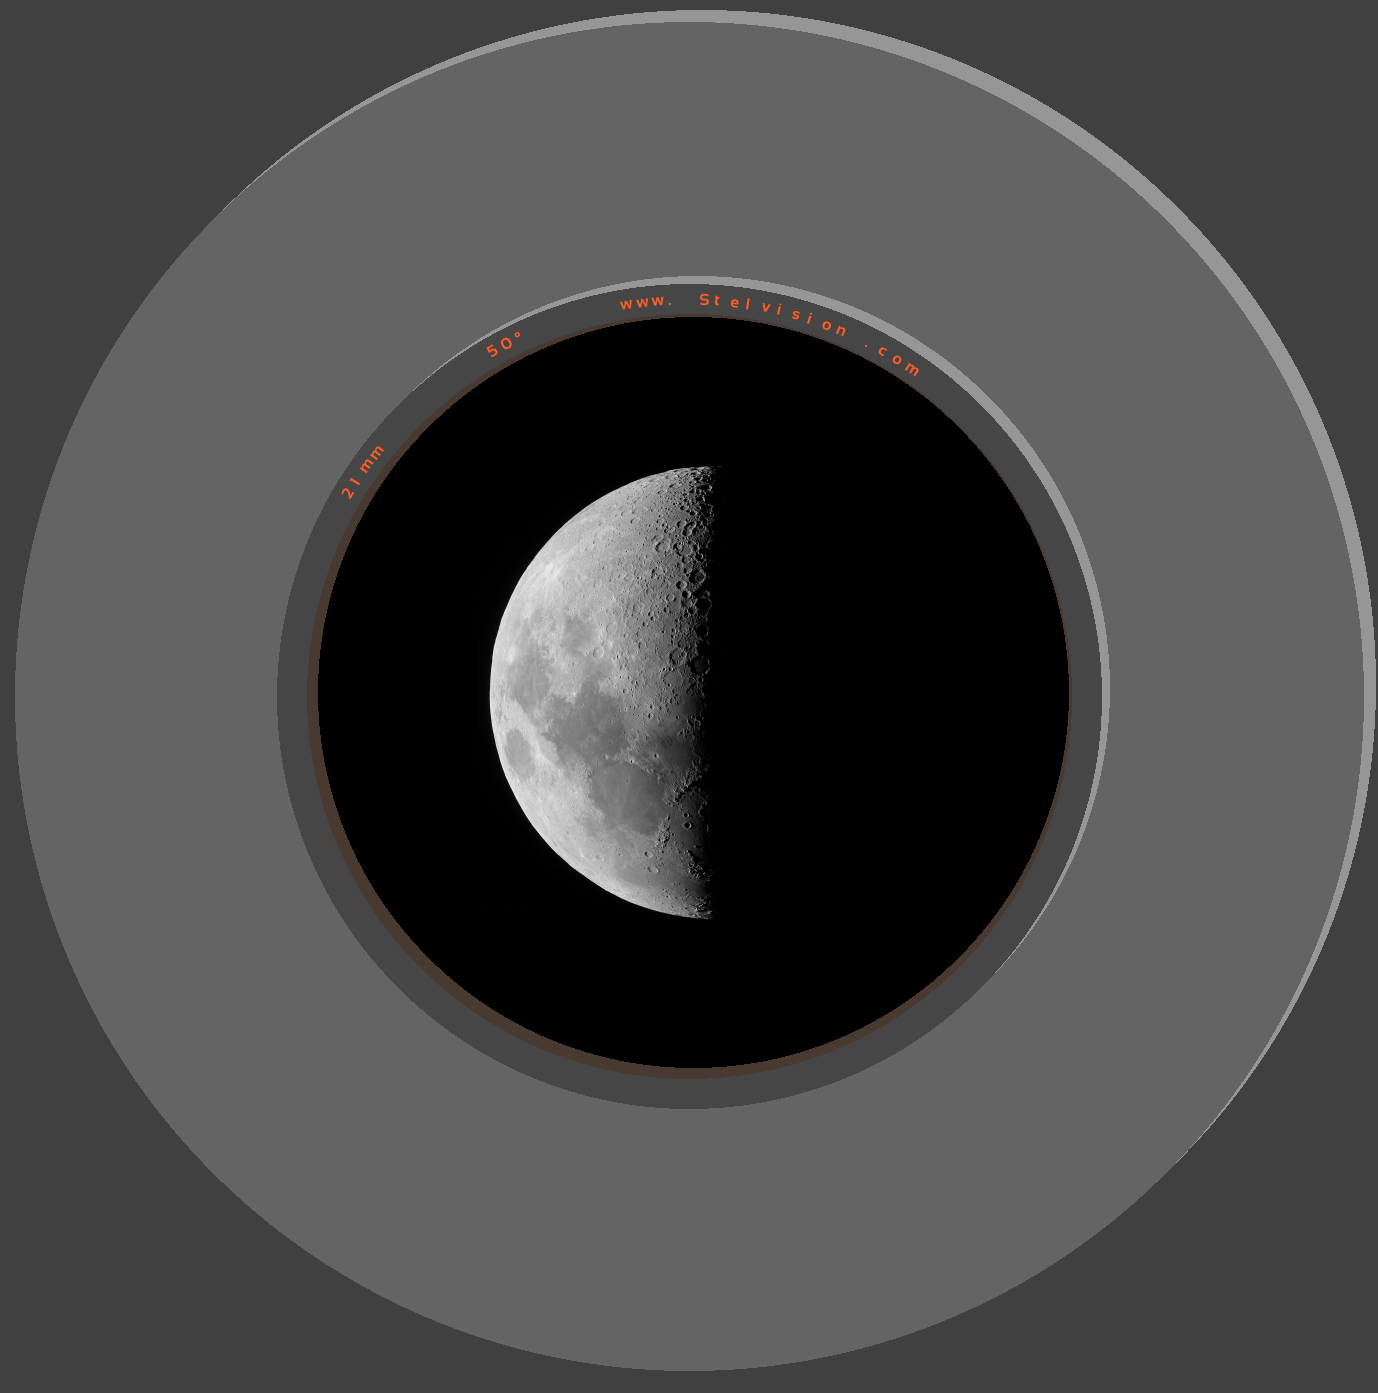
\includegraphics[width=0.30\linewidth]{\figures/photo_21lune.png}
    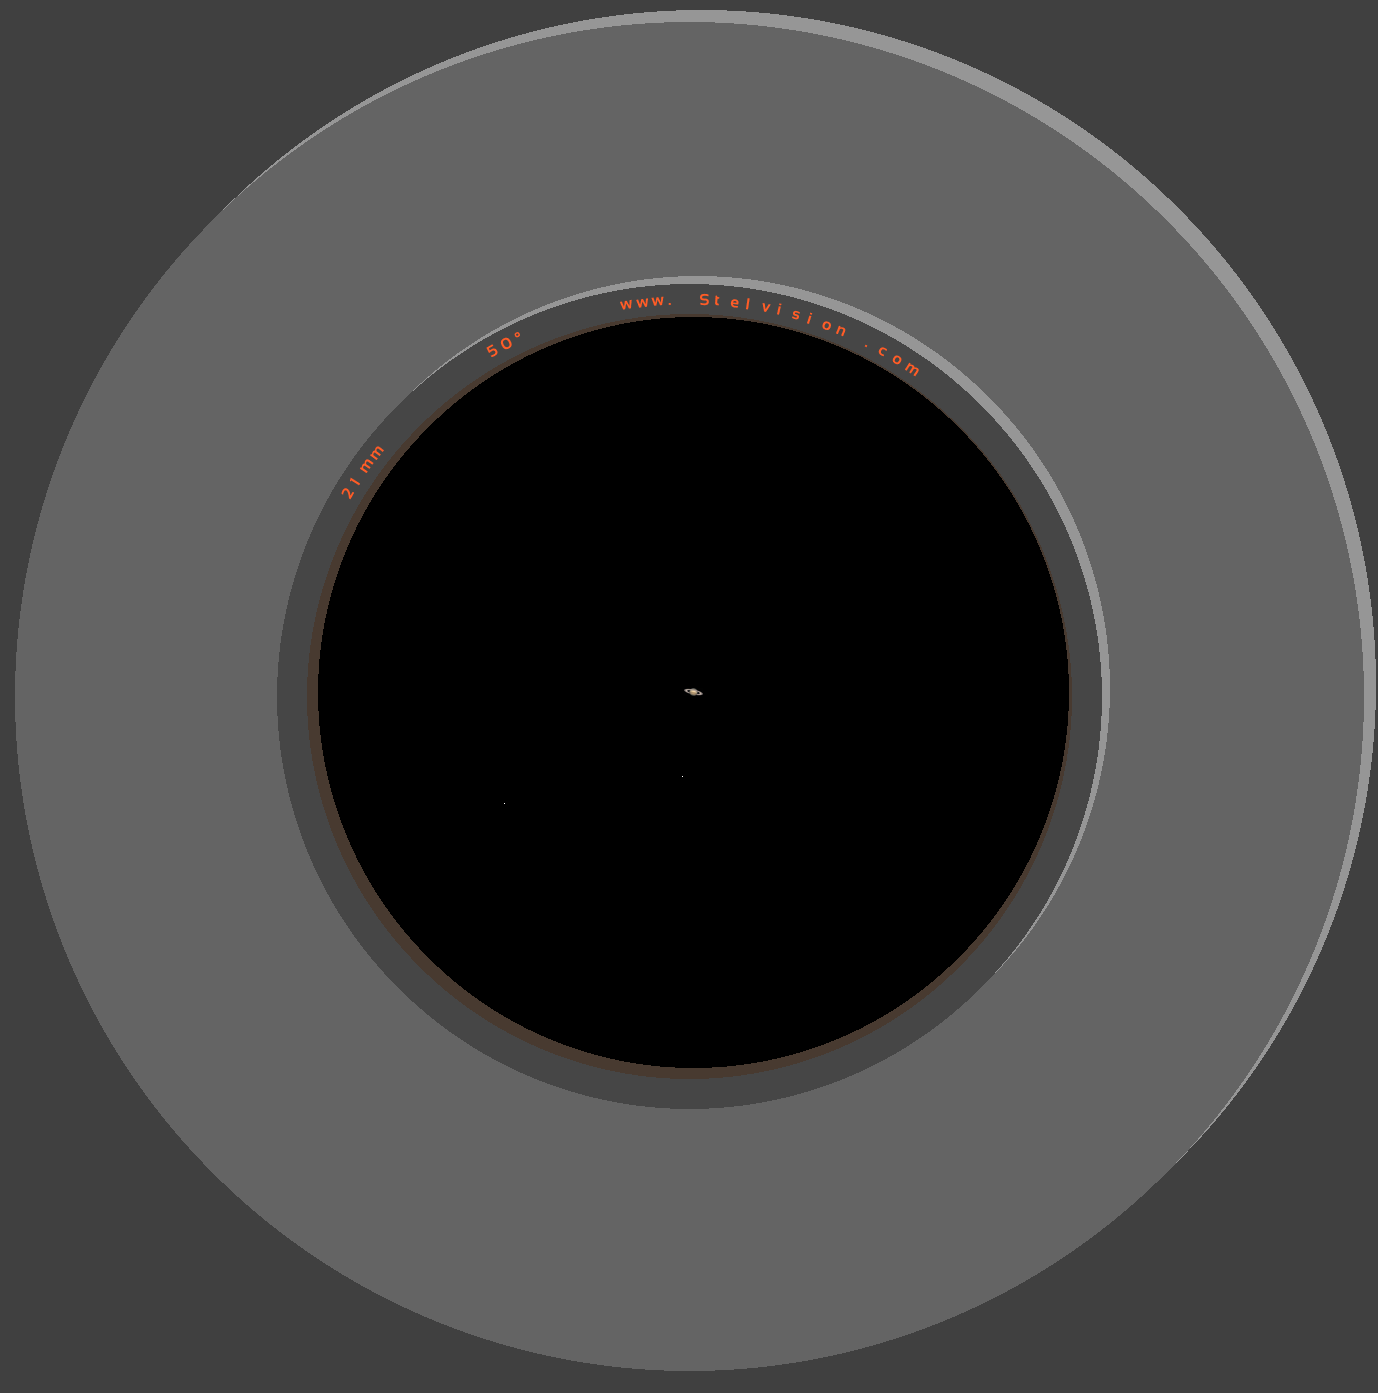
\includegraphics[width=0.30\linewidth]{\figures/photo_21saturne.png}
    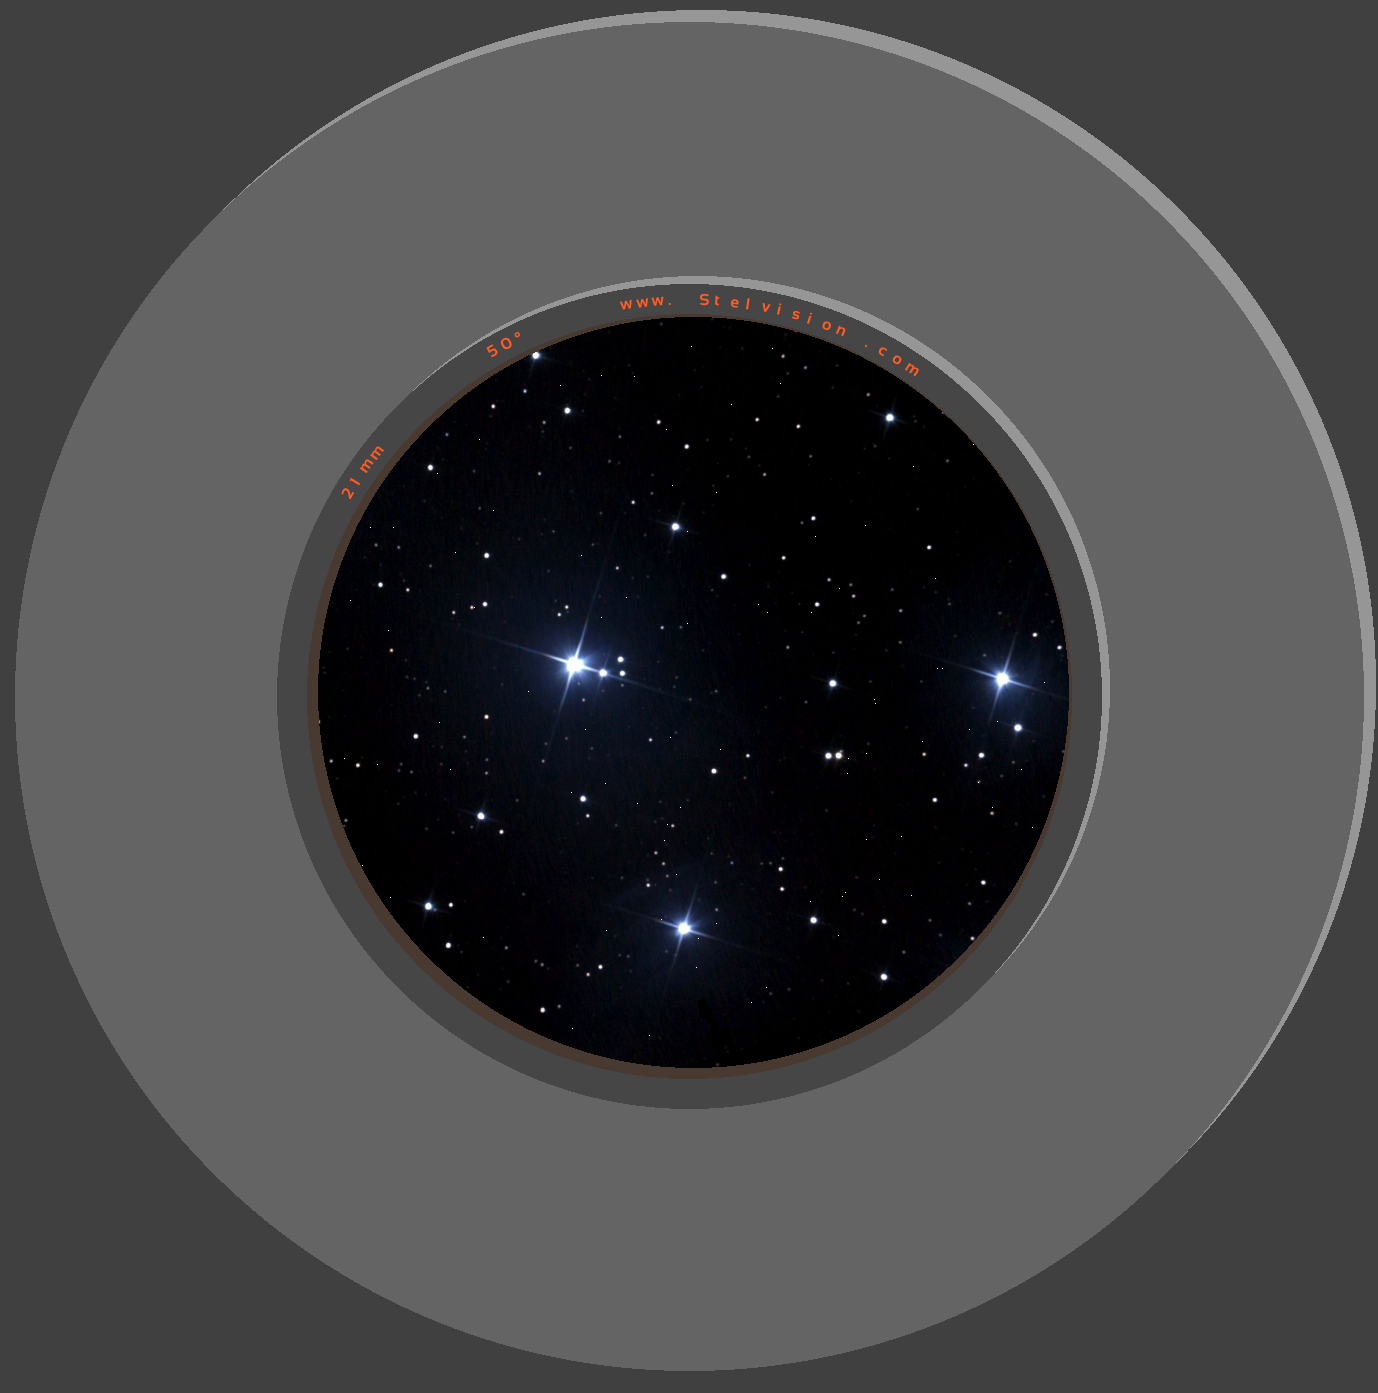
\includegraphics[width=0.30\linewidth]{\figures/photo_21pleiades.png}
    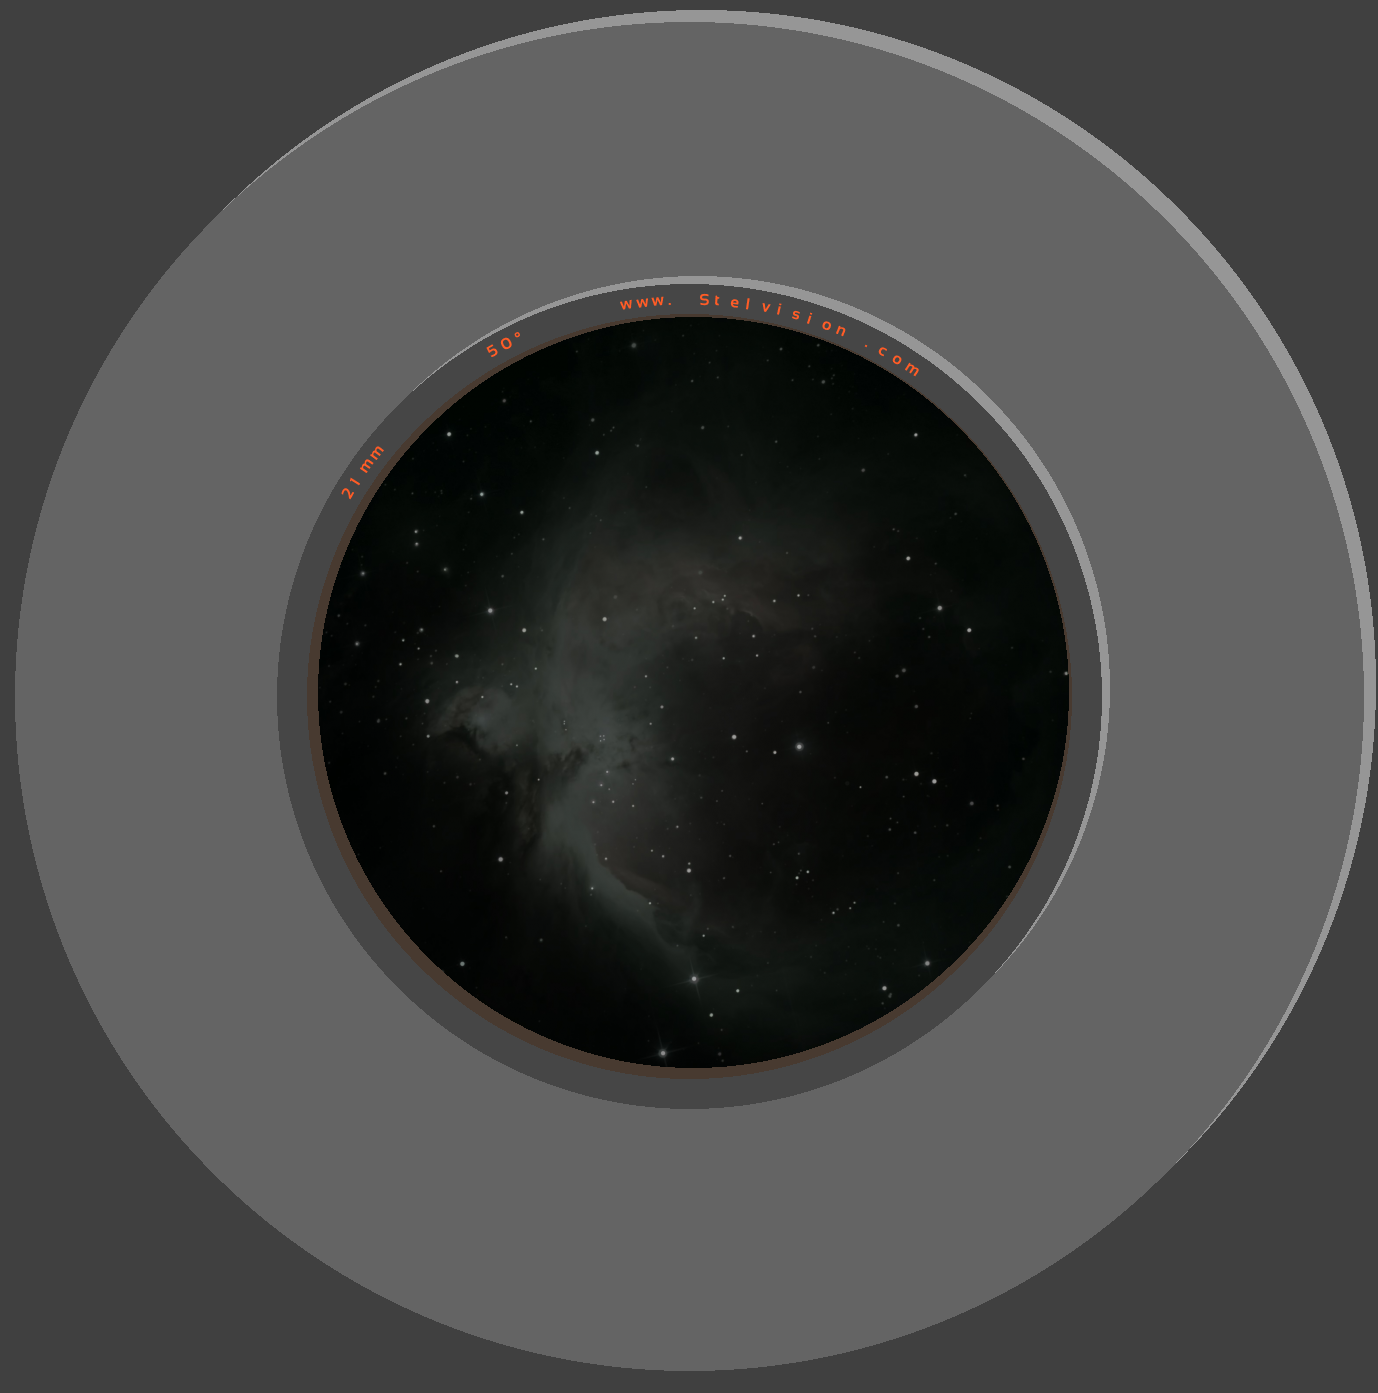
\includegraphics[width=0.30\linewidth]{\figures/photo_21m42.png}
    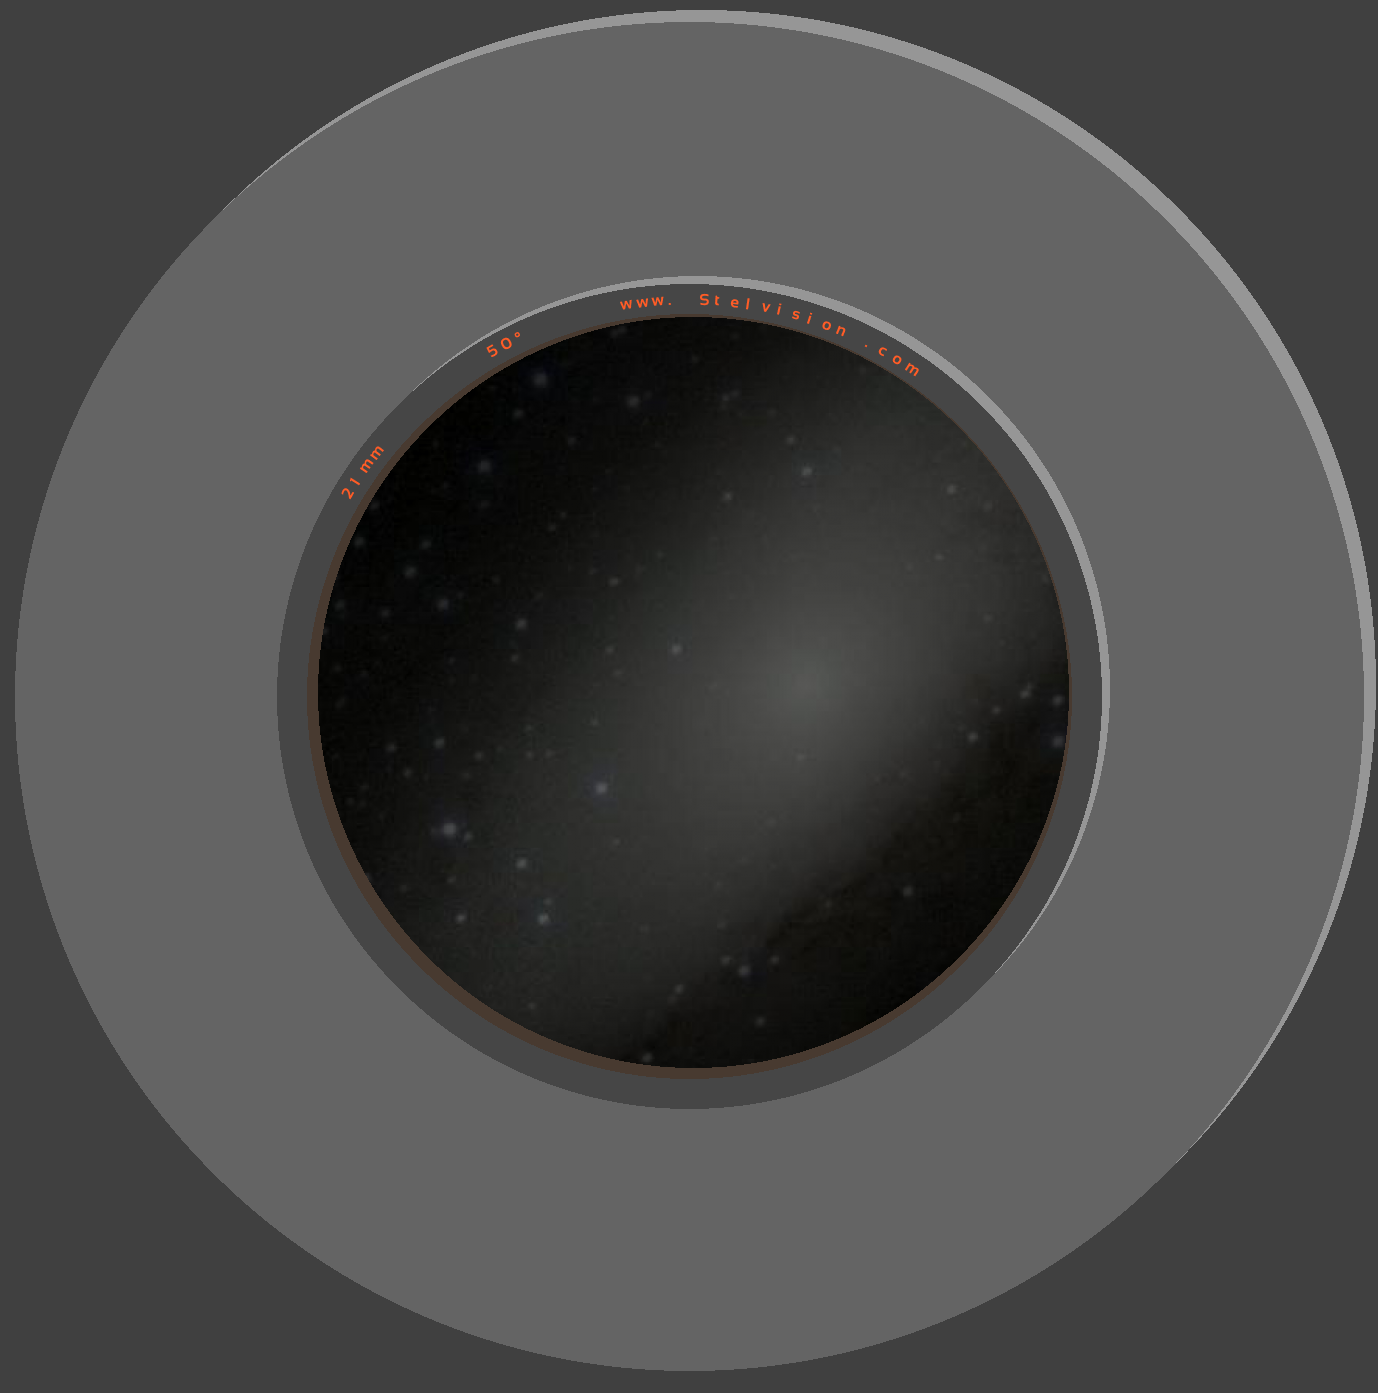
\includegraphics[width=0.30\linewidth]{\figures/photo_21m31.png}
    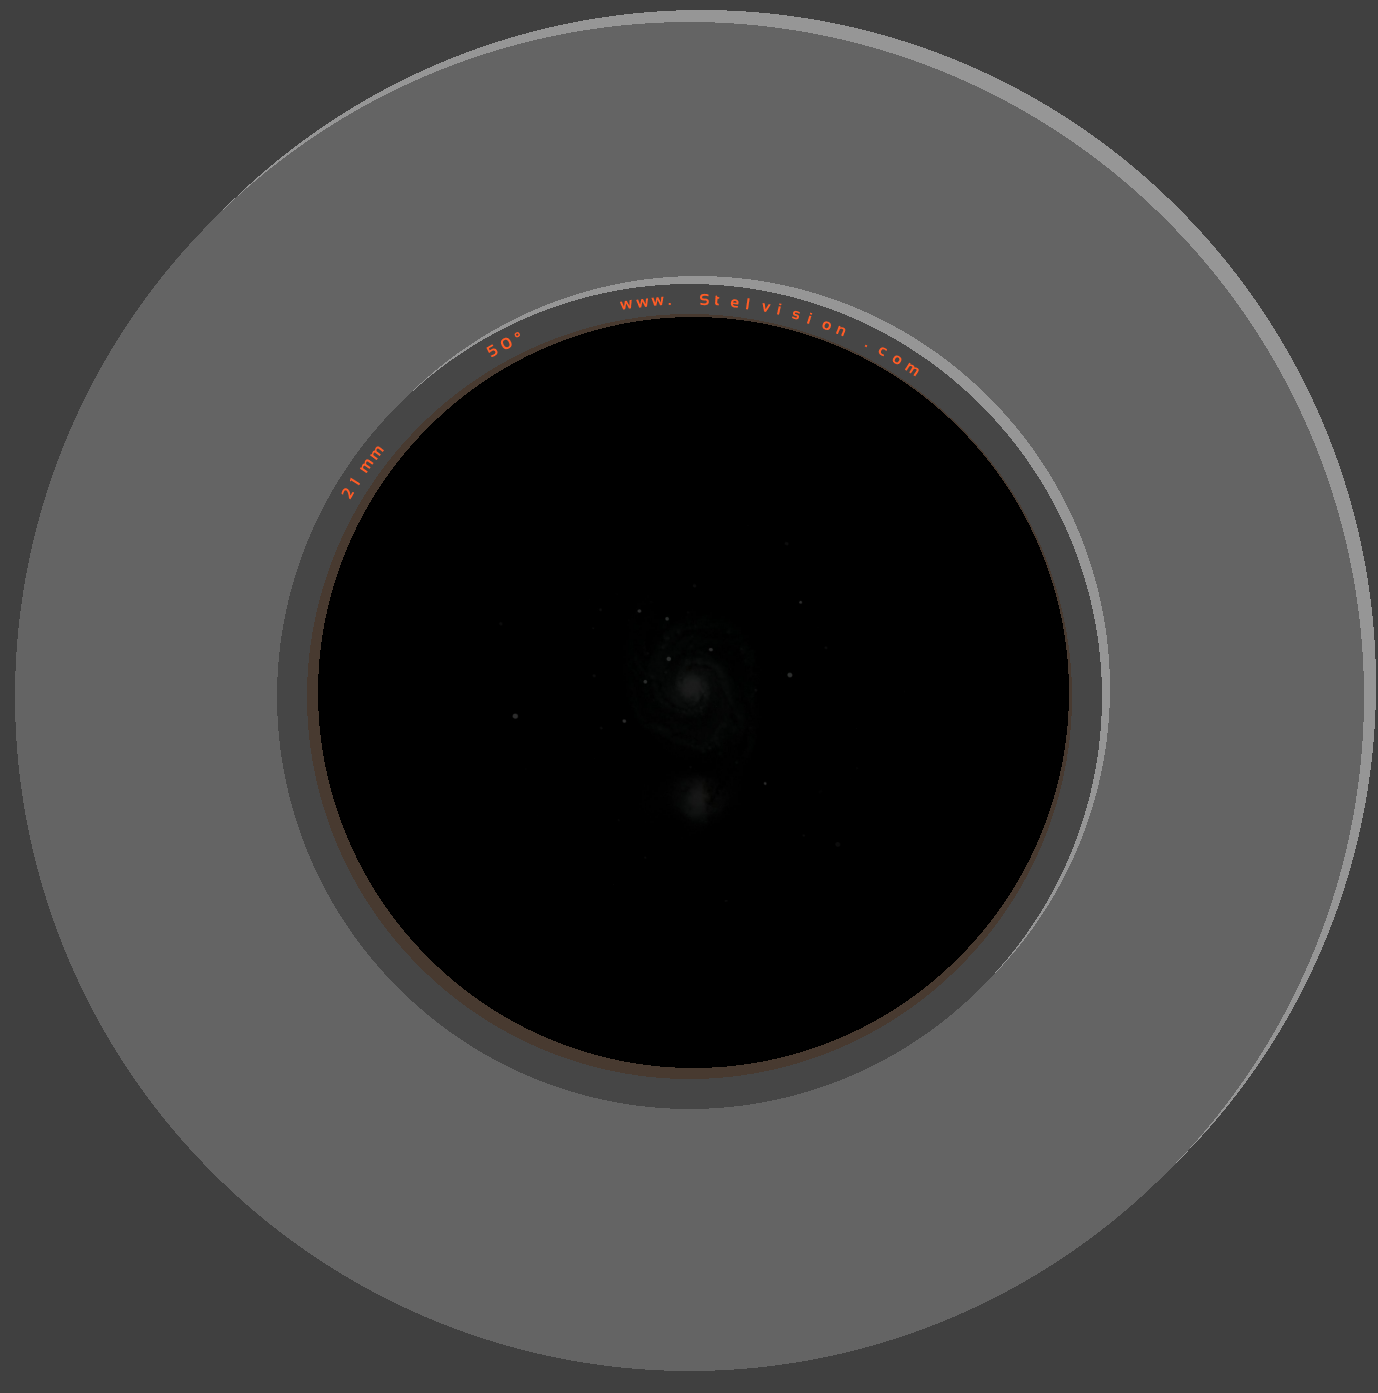
\includegraphics[width=0.30\linewidth]{\figures/photo_21m51.png}
    \decoRule
    \caption[
	Résultats de simulation pour un oculaire de focale $f=21mm$\\Lune, Saturne, les Pléiades,\\galaxies M42, M31, M51]{
	Résultats de simulation pour un oculaire de focale $f=21mm$\\Lune, Saturne, les Pléiades,\\galaxies M42, M31, M51}
    \label{fig:	Résultats de simulation pour un oculaire de focale $f=21mm$ Lune, Saturne, les Pléiades, galaxies M42, M31, M51}
    \end{figure}

\begin{figure}[H]
    \centering
    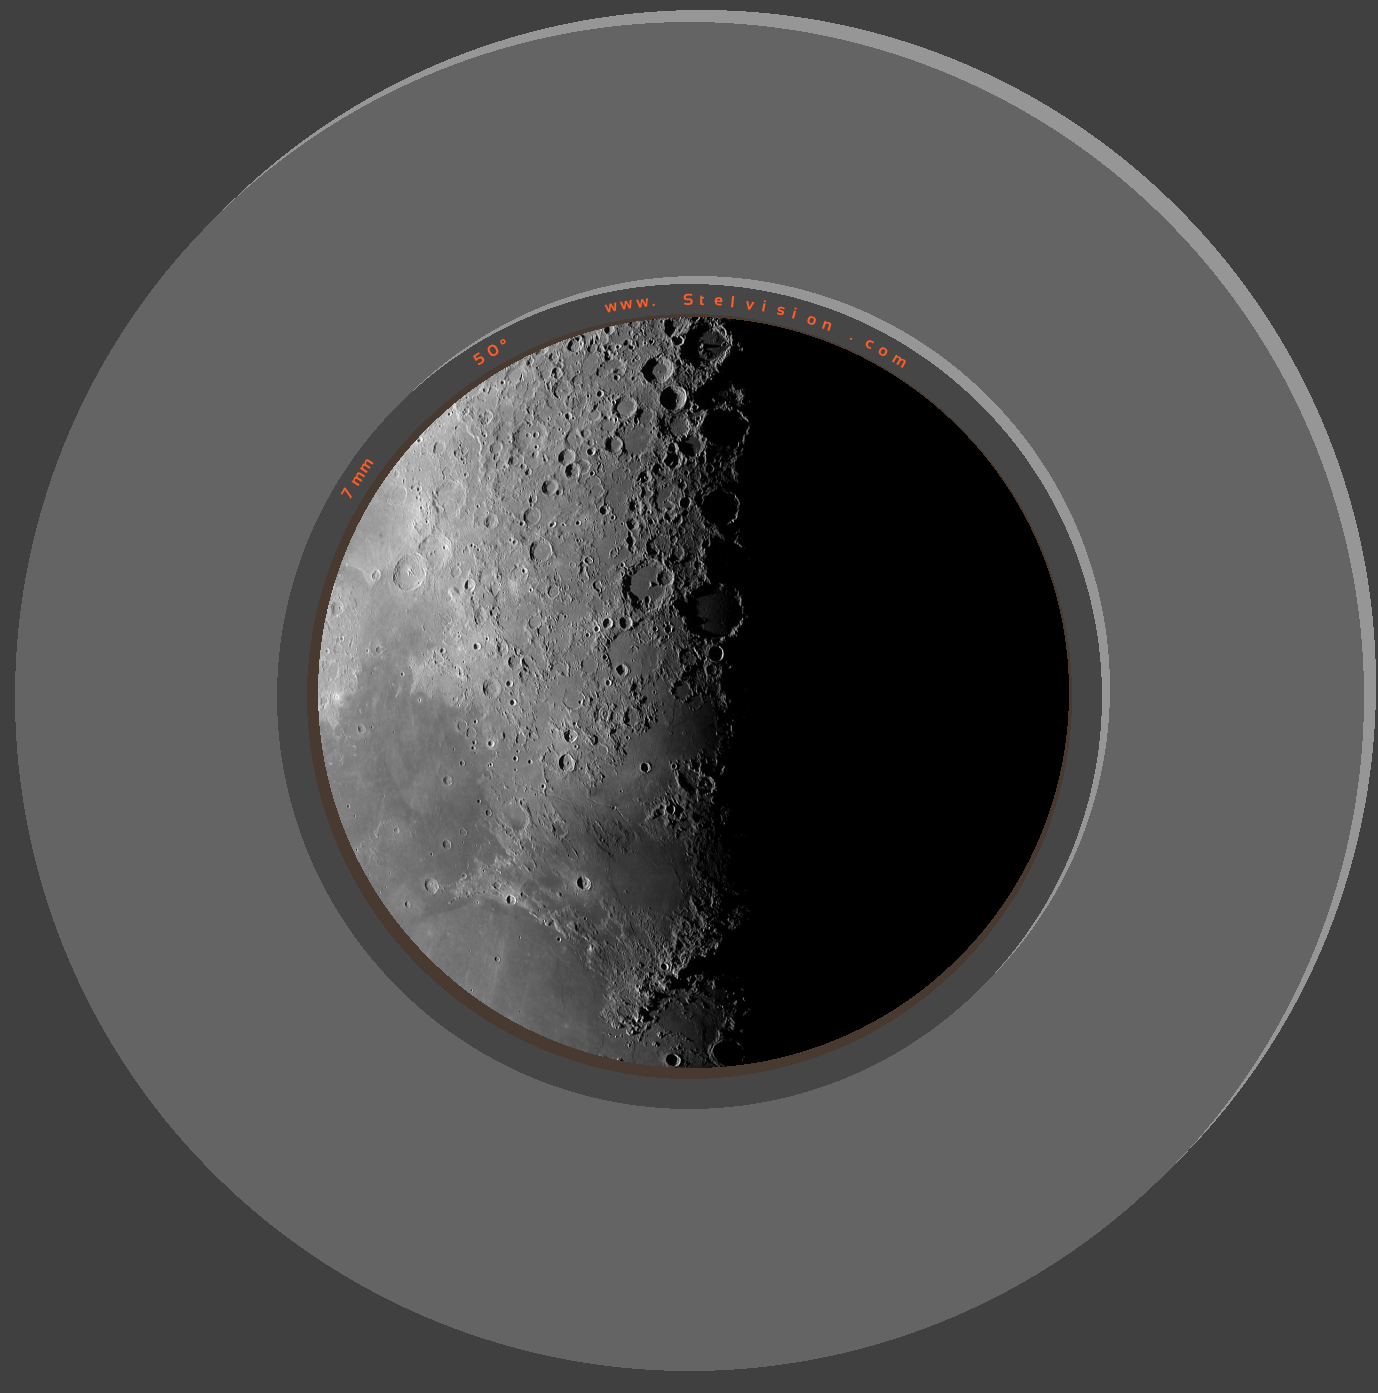
\includegraphics[width=0.30\linewidth]{\figures/photo_7lune.png}
    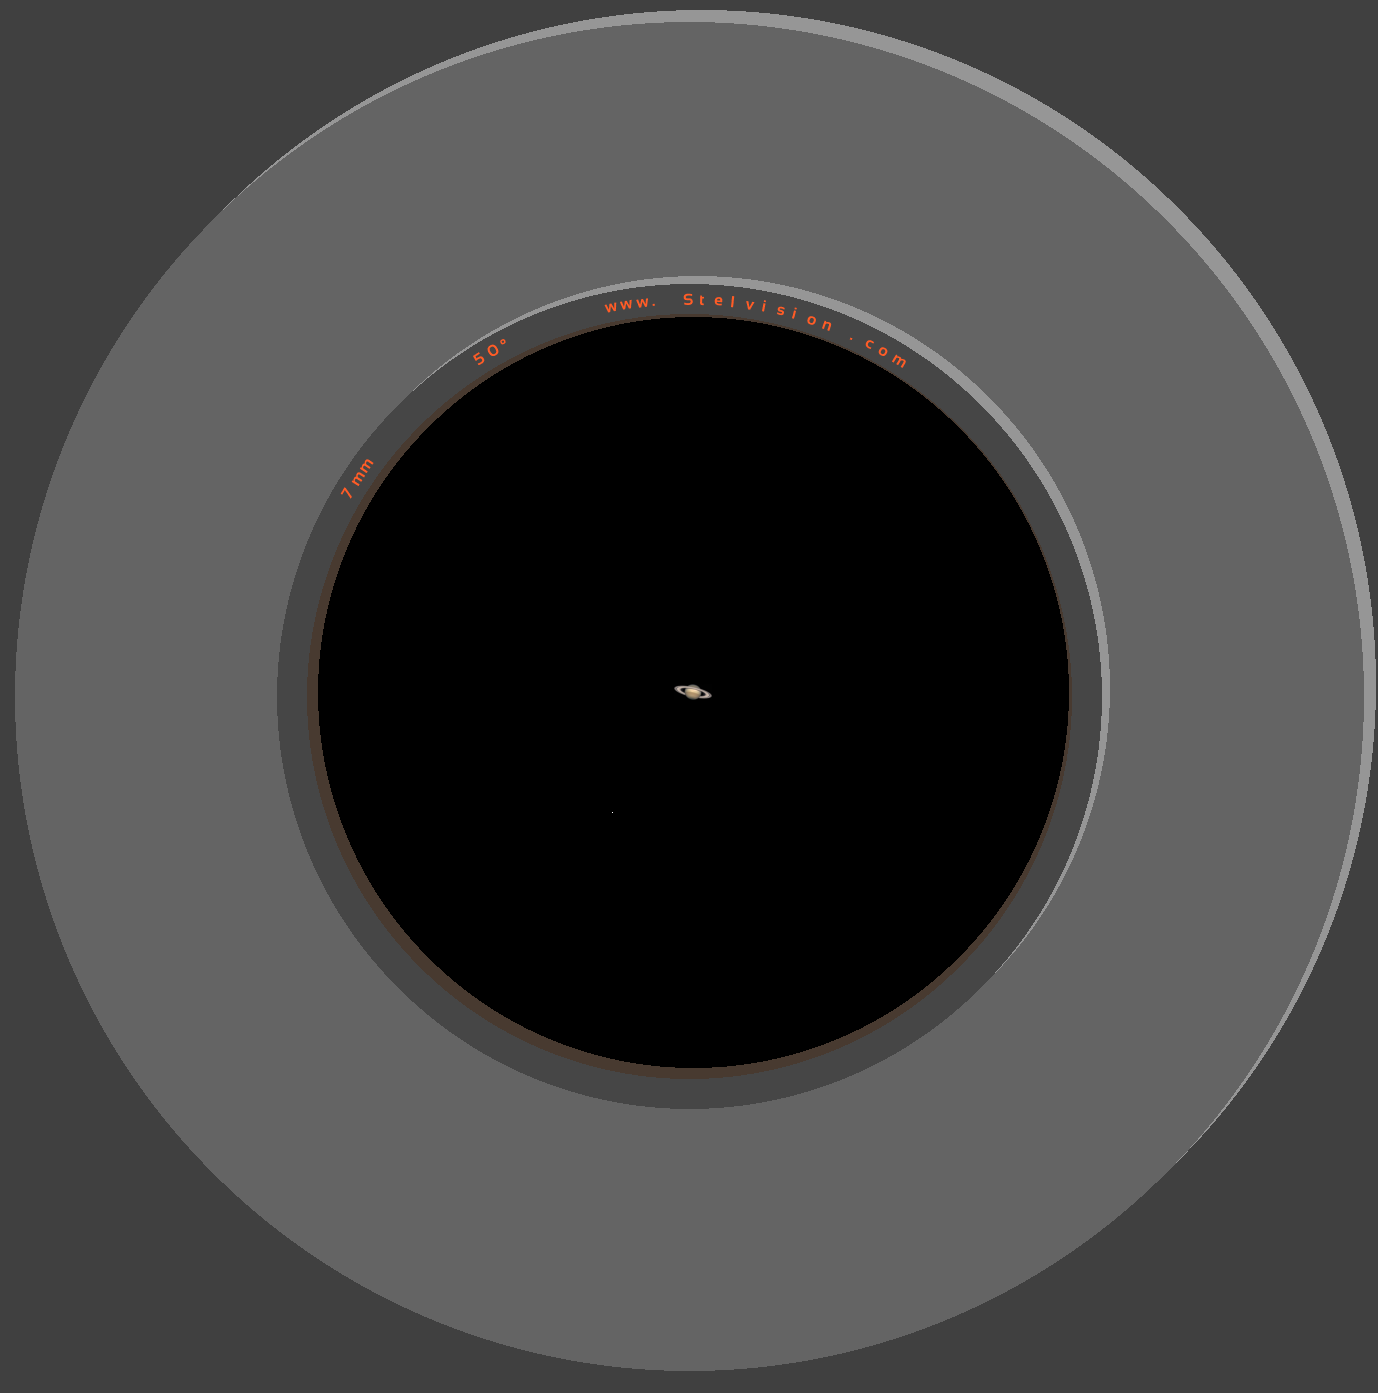
\includegraphics[width=0.30\linewidth]{\figures/photo_7saturne.png}
    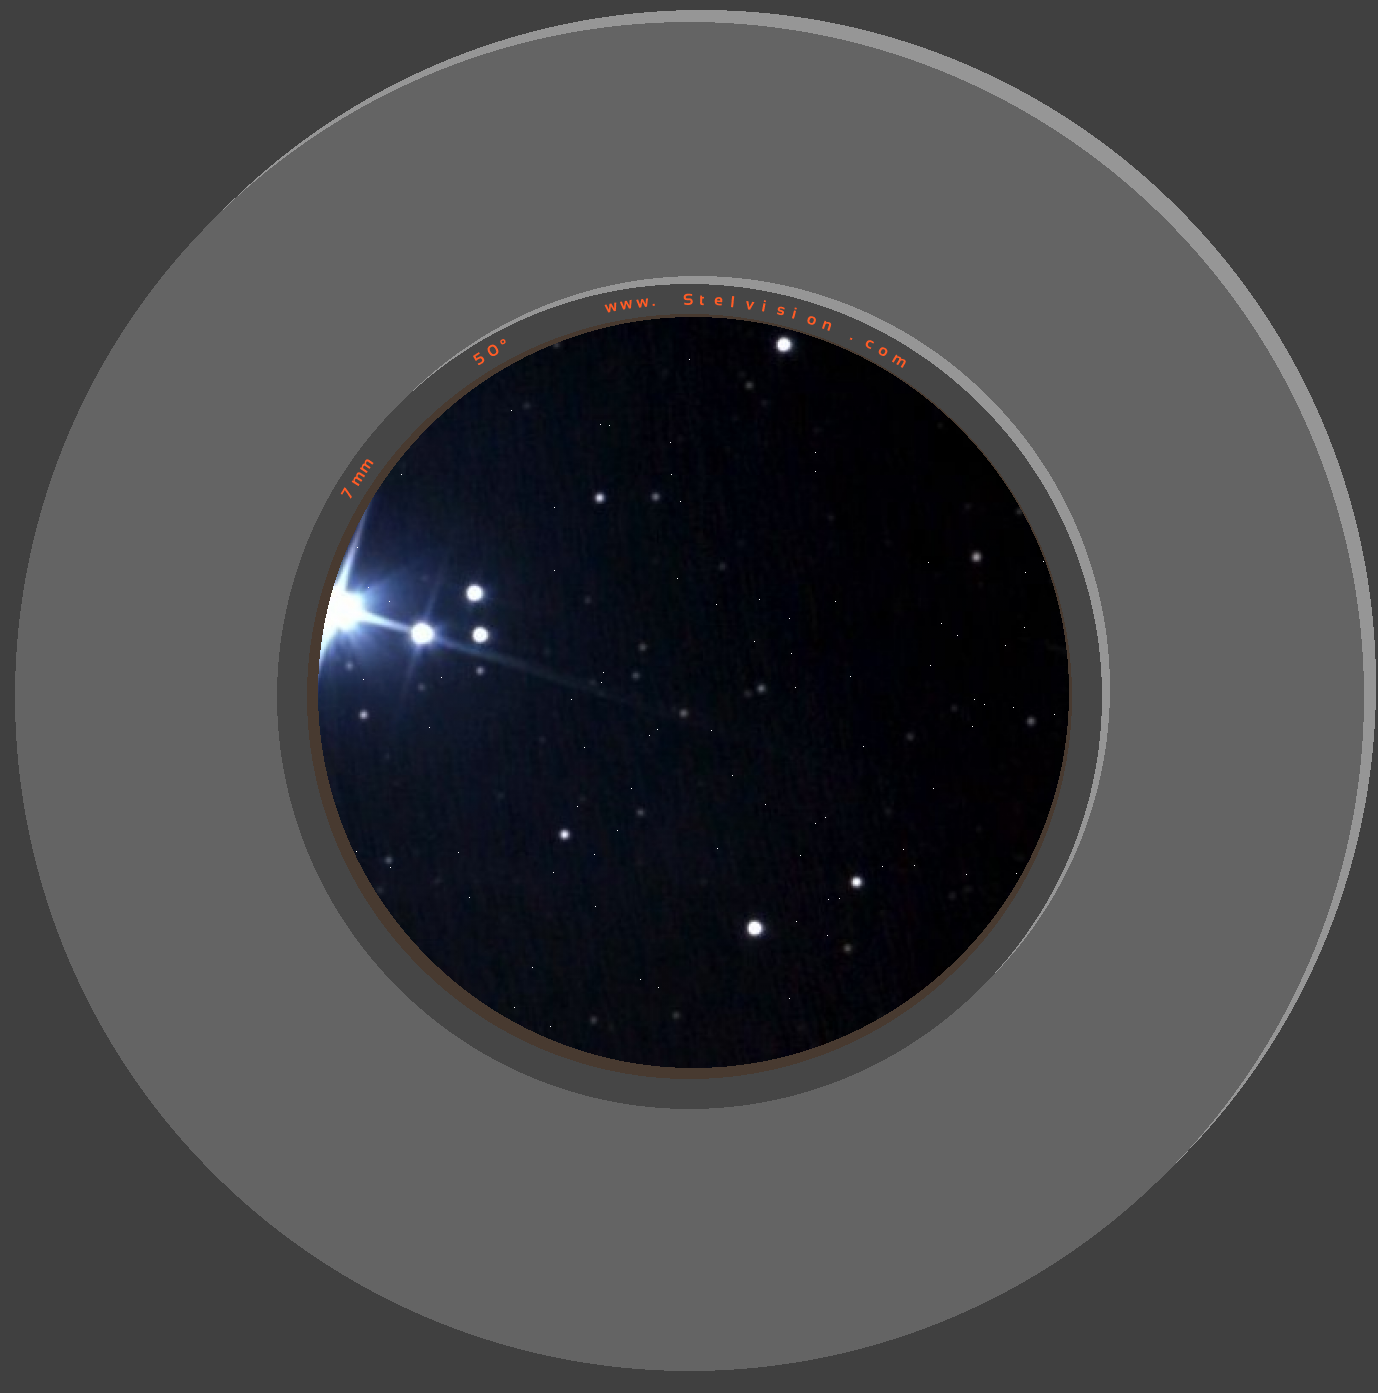
\includegraphics[width=0.30\linewidth]{\figures/photo_7pleiades.png}
    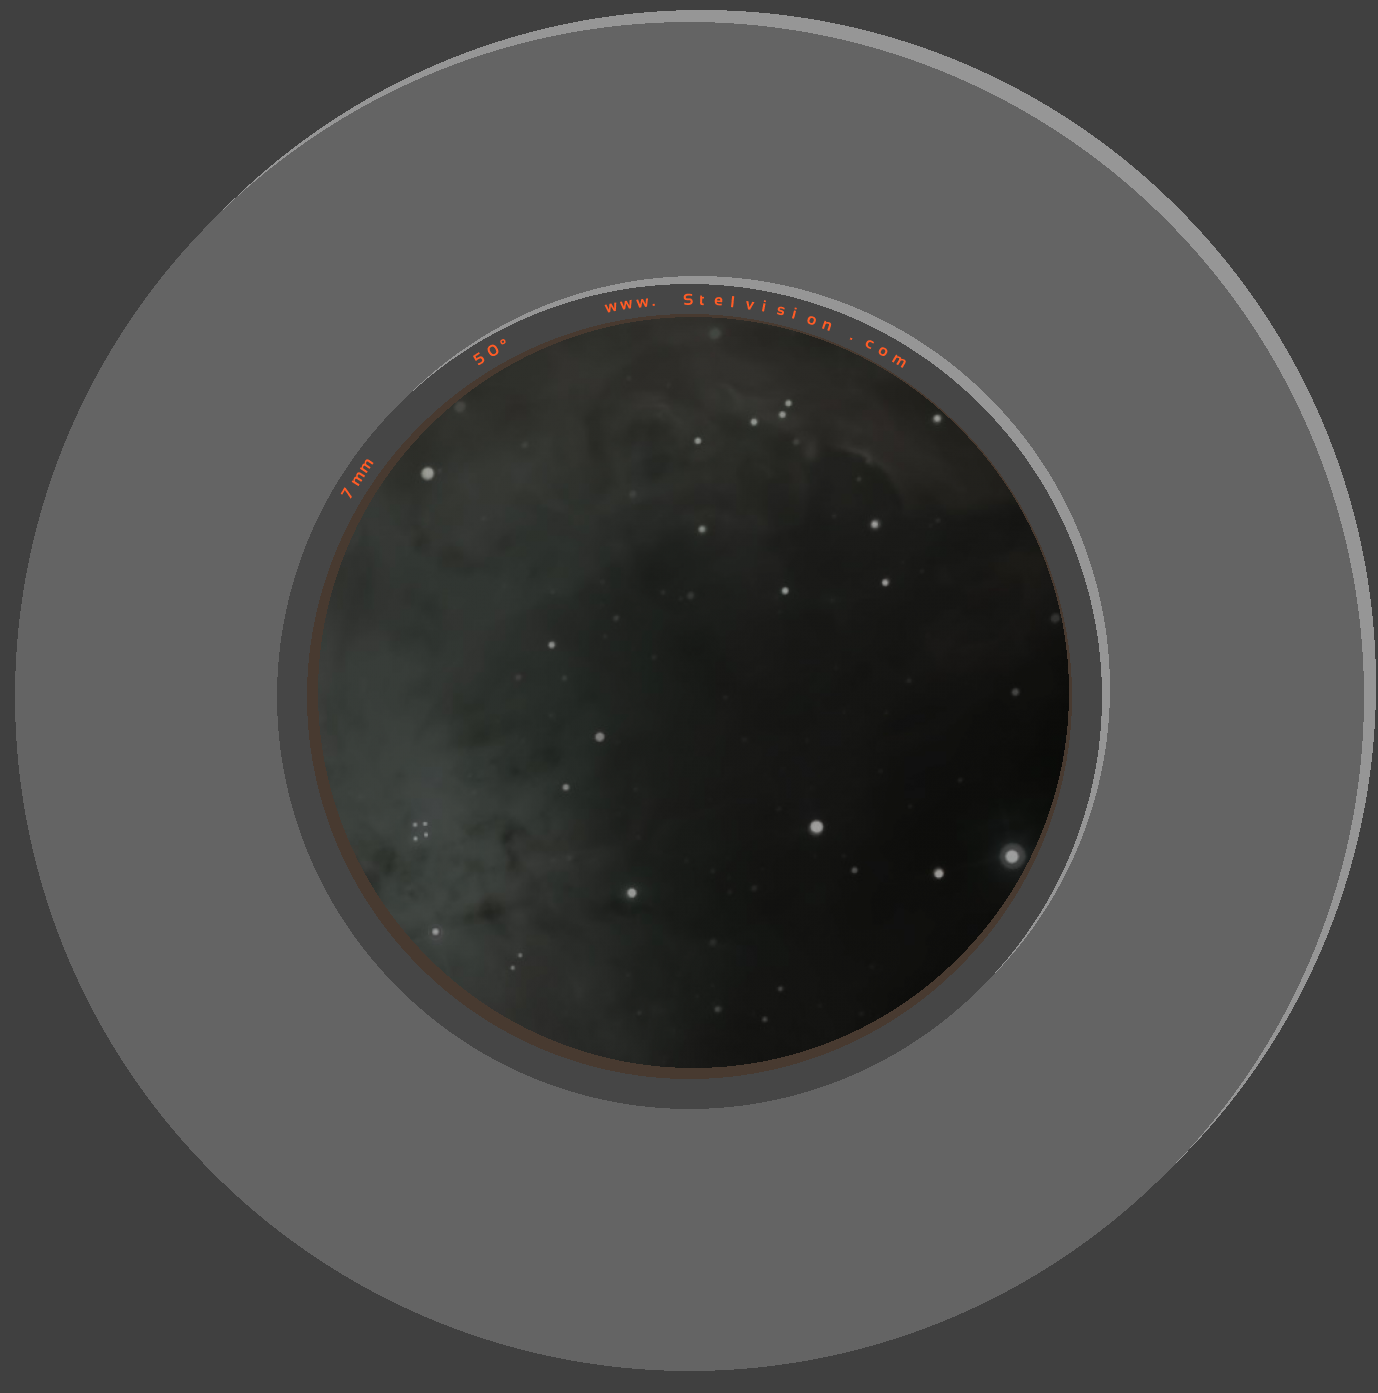
\includegraphics[width=0.30\linewidth]{\figures/photo_7m42.png}
    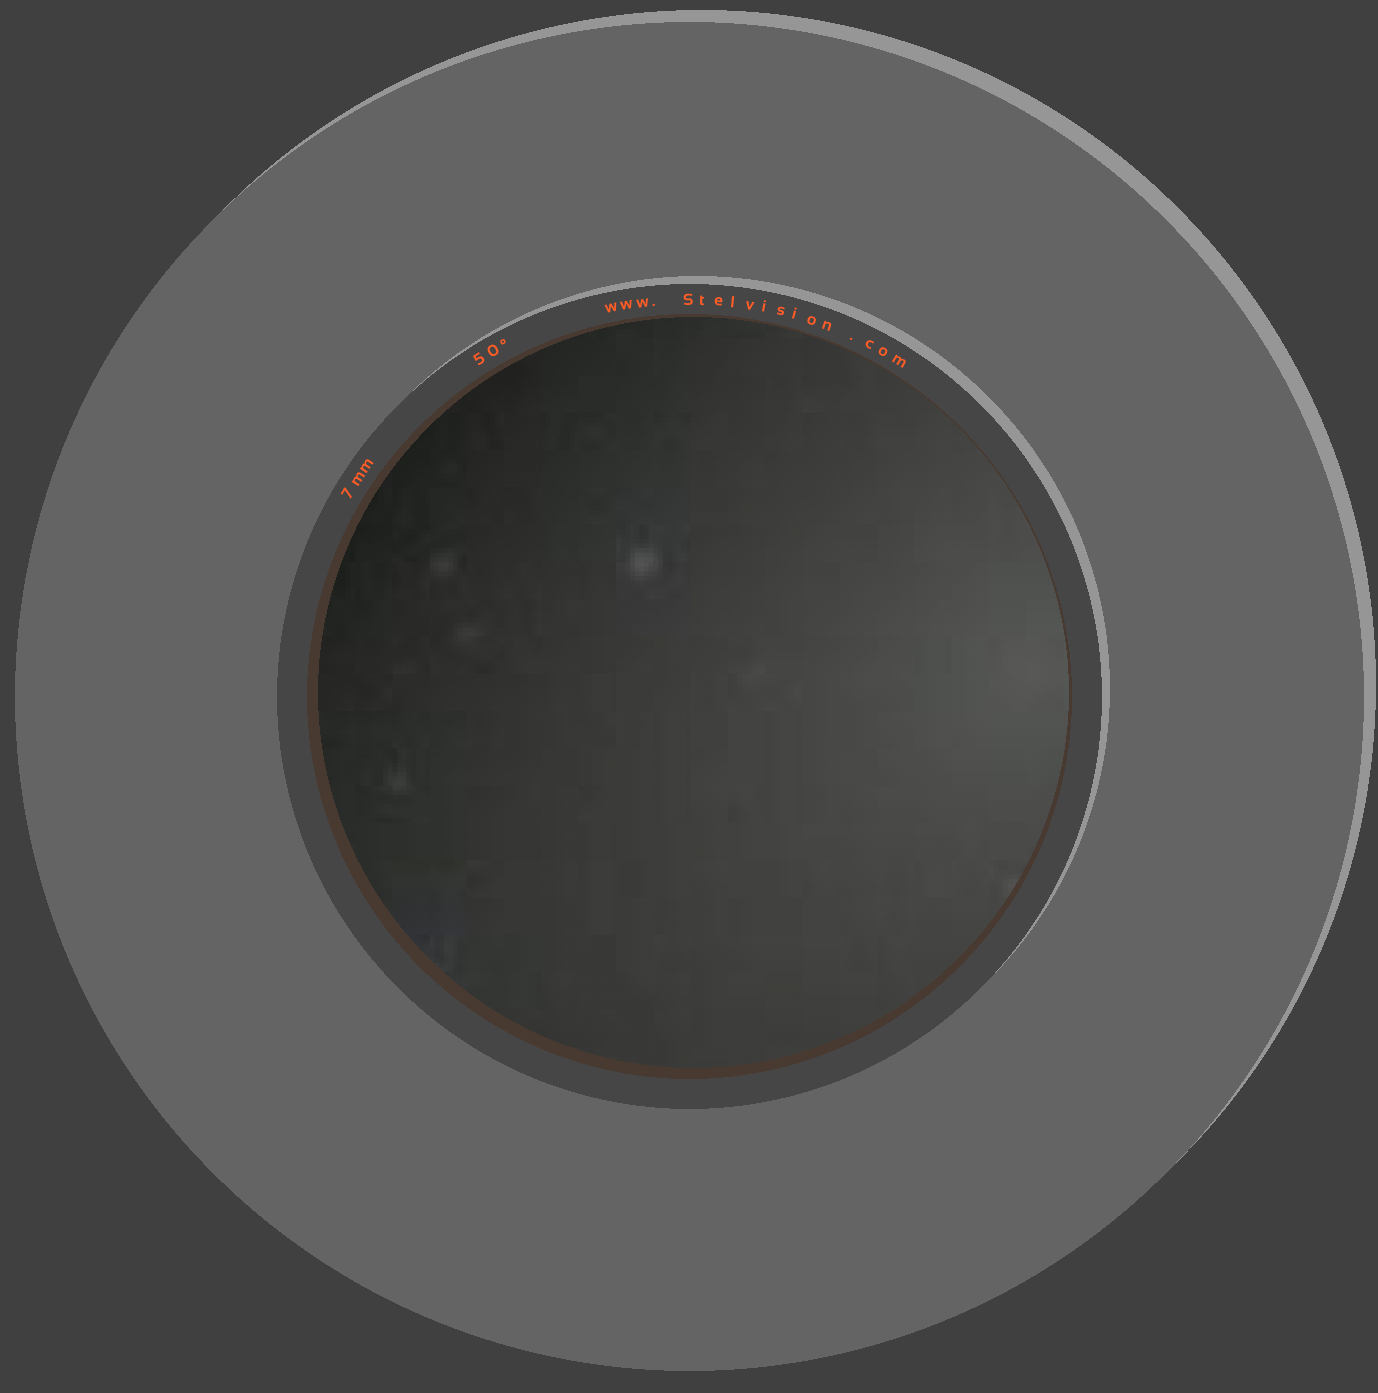
\includegraphics[width=0.30\linewidth]{\figures/photo_7m31.png}
    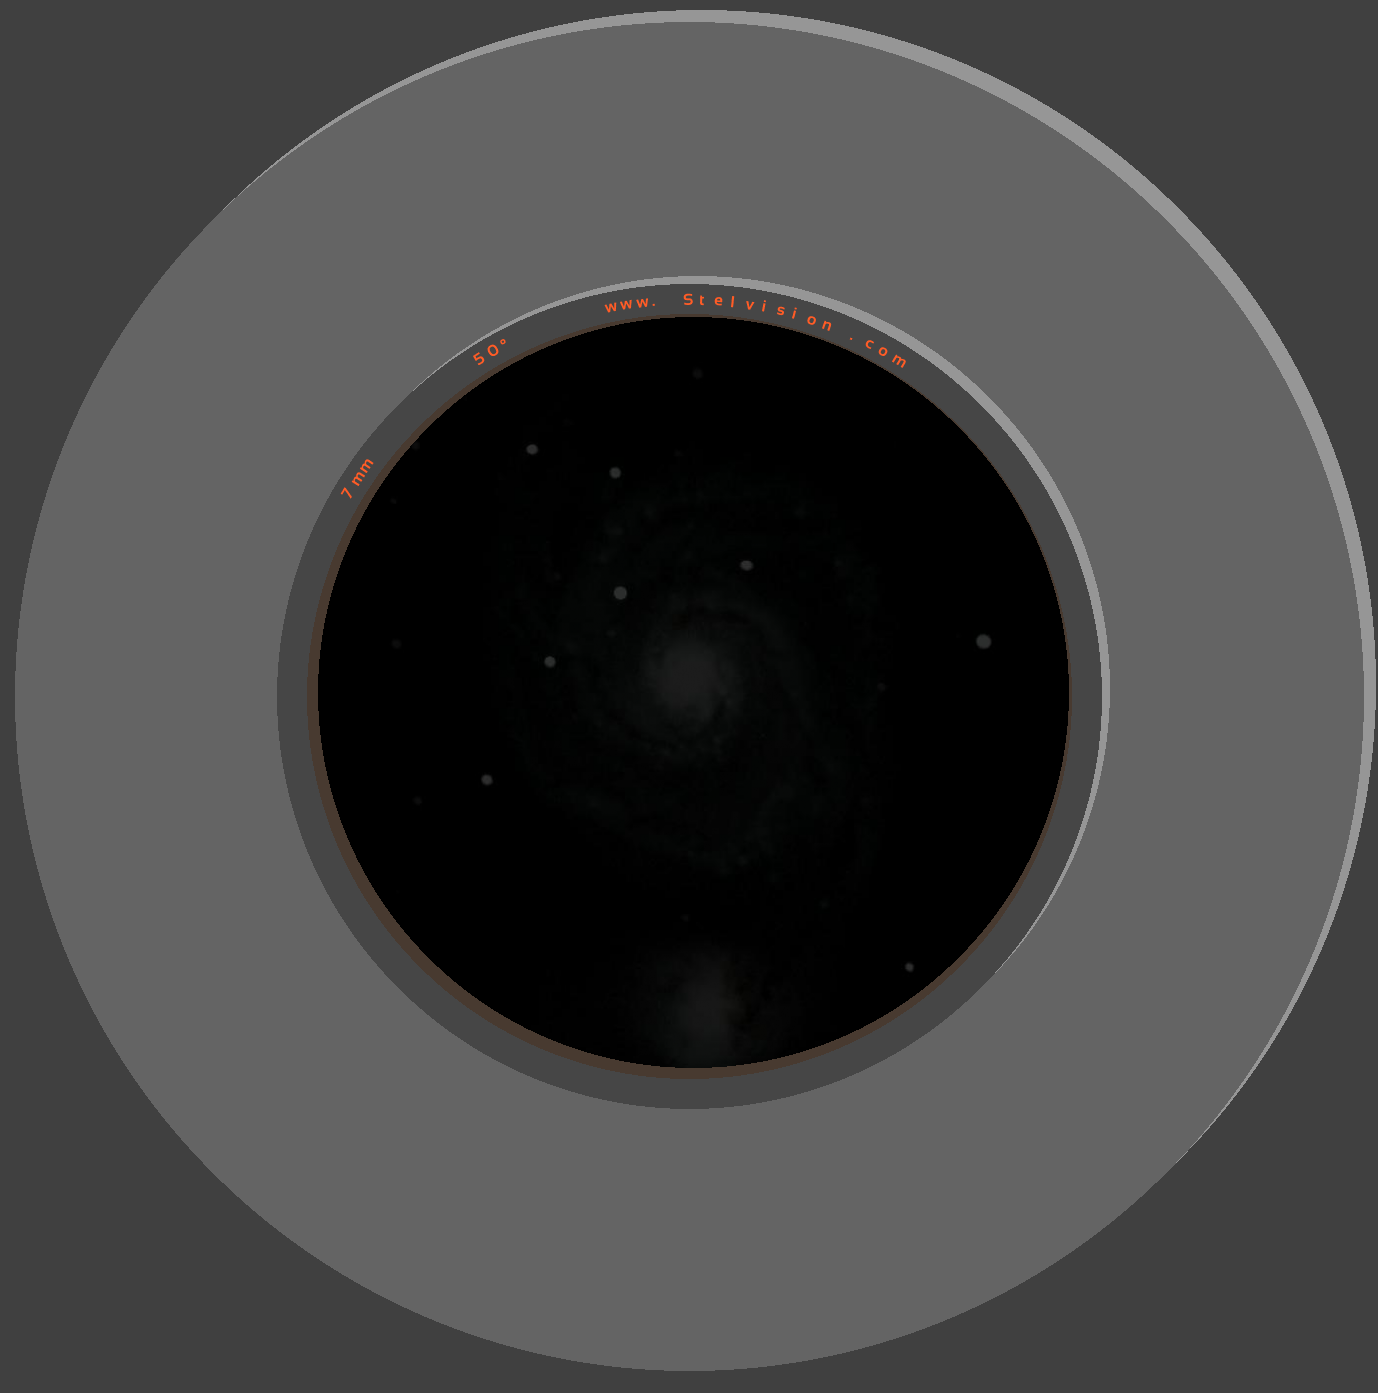
\includegraphics[width=0.30\linewidth]{\figures/photo_7m51.png}
    \decoRule
    \caption[
	Résultats de simulation pour un oculaire de focale $f=7mm$\\Lune, Saturne, les Pléiades,\\galaxies M42, M31, M51]{
	Résultats de simulation pour un oculaire de focale $f=7mm$\\Lune, Saturne, les Pléiades,\\galaxies M42, M31, M51}
    \label{fig:	Résultats de simulation pour un oculaire de focale $f=7mm$ Lune, Saturne, les Pléiades, galaxies M42, M31, M51}
    \end{figure}

\vspace{1cm}


L'oculaire zoom choisi est polyvalent et permet un compromis satisfaisant entre grossissement et luminosité / vue d'ensemble.

\url{https://www.astroshop.de/fr/oculaires/omegon-7-21mm-super-ploessl-oculaire-zoom-apo-1-25-/p,5084}

\begin{figure}[H]
    \centering
    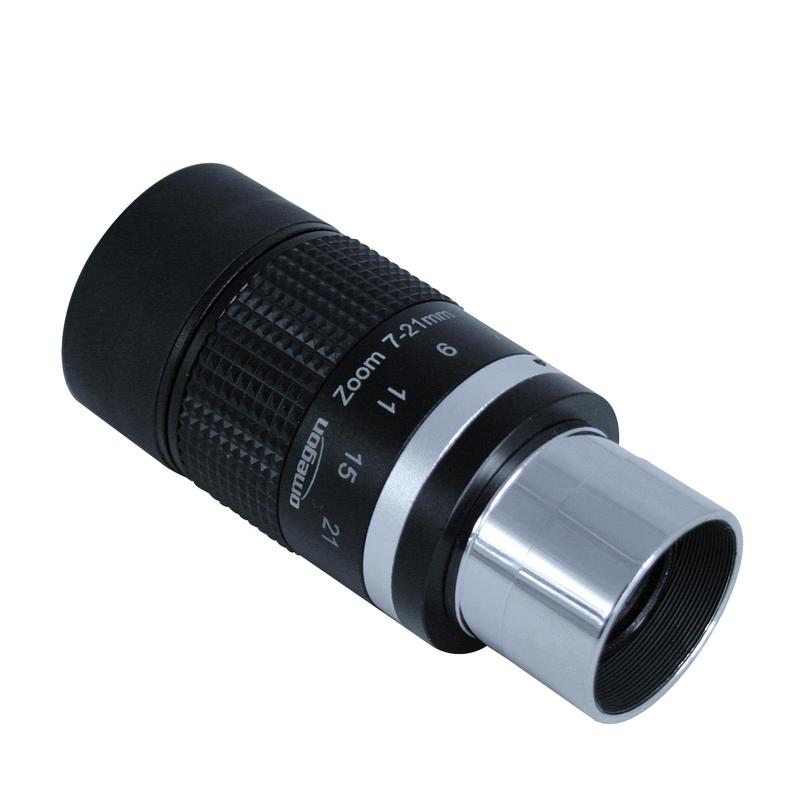
\includegraphics[width=0.5\linewidth]{\figures/photo_zoom.png}
    \decoRule
    \caption[
    Oculaire zoom $21mm-7mm$]{
    Oculaire zoom $21mm-7mm$}
    \label{fig:Oculaire zoom $21mm-7mm$}
    \end{figure}
